
This chapter introduces test statistic inversion as a method of estimating confidence intervals and outlines several inversion-based approaches for estimating extinction times. This chapter also introduces a new inference approach called Min-MI, which can be used to estimate extinction time using the sample minimum statistic.

\section{Test Inversion Confidence Intervals}

We first introduce test statistic inversion as a method for constructing confidence intervals for an unknown parameter $\theta \in \R$ \parencite{Carpenter1999}. Let $\bm{X}$ denote a random vector of $n$ independent and identically distributed random variables from a distribution with CDF $F_X (\cdot; \theta)$. Let $S(\bm{X})$ be a consistent estimator of $\theta$. Denote $\bm{x}$ and $S(\bm{x})$ be a realisation of $\bm{X}$ and $S(\bm{X})$ respectively, and let $\alpha$ be a fixed significance level for the test. Suppose $S$ is stochastically increasing with $\theta$:

\begin{equation}
    \theta_1 < \theta_2 \implies F_S(\theta_1) < F_S(\theta_2) 
\end{equation}

where $F_S(\theta) = \PP_\theta\left\{S(\bm{X}) > S(\bm{x})\right\}$. Then, a central $100(1-\alpha)\%$ confidence interval denoted by $[L, U]$ can be found, where $L$ and $U$ satisfy: \begin{equation}
\begin{aligned}
    \PP_{\theta = L}\left\{S(\bm{X}) > S(\bm{x})\right\} &= \alpha/2 \\
    \PP_{\theta = U}\left\{S(\bm{X}) > S(\bm{x})\right\} &= 1 - \alpha/2
\end{aligned}
\end{equation}

More generally, this method can be used to find the $q$\textsuperscript{th} quantile of $\theta$, $\theta_q$: \begin{equation}\label{eq: inversion}
    \PP_{\theta = \theta_q}\left\{S(\bm{X}) > S(\bm{x})\right\} = q
\end{equation}

This method of constructing confidence intervals exploits the duality between confidence intervals and hypothesis tests. Consider a two-sided test of the null hypothesis $H_0: \theta = \theta_0$ using test statistic $S(\bm{x})$. A $100(1-\alpha)\%$ confidence interval is the set of hypothesised values for $\theta_0$ where the test is not significant at level $\alpha$. The duality refers to the way $\theta_0$ is always in the $100(1-\alpha)\%$ confidence interval if the test is not significant at $\alpha$.

Thus, by inverting the test's acceptance region so that the region is a function of $\theta$ rather than being a function of the test-statistic, a confidence interval may be constructed. This naturally relies on a monotonocity assumption, as inversion is only valid where $S$ is stochastically increasing with $\theta$.

\section{Simulated-Inversion Estimator}

We now describe the simulated-inversion (SI) estimator, a method proposed by \textcite{Huang2019}. This method assumes a data generation process following model $M$, which may or may not account for measurement error. The goal is to estimate $\PP_\theta\left\{S(\bm{X}) > S(\bm{x})\right\}$ by simulation, and then construct confidence intervals by inversion. These two steps are described below:

\begin{enumerate}
    \item \textbf{Simulation}: Suppose we have a given dataset $\bm{x} = [x_1, x_2, \dots, x_n]^\top$ and a known set of $r$ potential values for the true extinction time $\bm{\theta} = [\theta_1, \theta_2, \dots, \theta_r]^\top$. Then, for each potential value $\theta_i$, simulate a pseudo dataset $\bm{x}^*_i$ from the model $M$ specified by $\theta_i$ and take a sample statistic $S^*_i$ from the pseudo dataset. Thus, for a given dataset of $n$ observations and a set of $r$ potential values for $\theta$, a set of $r$ simulated statistics $\bm{S}^*$ can be obtained.
    \item \textbf{Inversion}: An estimate for $\PP_\theta\left\{S(\bm{X}) > S(\bm{x})\right\}$ is constructed by regressing the indicator $\mathbbm{1}\left\{ S(\bm{X}^*_i) > S(\bm{x}^*_i) \right\}$ against $\theta_i$ for all $i \in \left\{ 1, \dots, r \right\}$. Finally, $\theta$ can be estimated by inverting the estimated curve.
\end{enumerate}

This method of extinction estimation lends itself to be fairly general, as it only requires a vector of potential values for $\theta$, a stochastically increasing statistic, and a simulation model. Thus, the SI estimator can be used regardless of a uniform distribution assumption and can also account for the presence of measurement errors.

That being said, there are some disadvantages to the SI estimator. Since the true extinction time is unknown, the interval of potential values for $\theta$ must necessarily be wide, and even wider where confidence intervals need to be constructed; resulting in fairly slow computation time in the absence of information to constrain the search interval. In the inversion step, the regression fit for $\PP_\theta\left\{S(\bm{X}) > S(\bm{x})\right\}$ may not necessarily be monotonic, and so this method could be improved by enforcing monotonicity, a conclusion supported by work done by \textcite{King2020}.

\section{Robbins-Monro (RM) Process}

We now propose applying the Robbins-Monro (RM) process, a classical stochastic approximation algorithm, to estimate extinction times. Although the RM process has not yet been used to search for extinction times and endpoints of confidence intervals in paleobiology, it is a generally well used technique in other spaces \parencite{Carpenter1999, Fisher2020}, and we draw from \textcite{Garthwaite1992}'s work to propose an inversion-based estimator for confidence intervals in a paleobiological context.

The RM process, or RM algorithm, was originally introduced to solve the rootfinding problem  \parencite{Fu2015}: \[ M(\theta)\overset{\text{def}}{=} \E_\theta H(\bm{X}) = \alpha \] for $X \in \R$, $\alpha \in \R$, $\E_\theta$ means expectation with respect to $\theta$, and $M(\theta)$ is a monotonically increasing function. The objective of the RM process is to find a sequence $\{\theta_n\}$ that converges to a unique (local) optimum $\theta^*$ by using the recursion \[ \theta_{i+1} = \theta_i - c_i \widehat{\nabla f}(\theta) \] where $c_i > 0$ is the step size. This recursion converges in mean square to the optimum $\theta^*$. Moreover, the step sizes $c_n$ must decrease according to conditions $\sum_nc_n^2 < \infty$ and $\sum_n c_n = \infty$.

\textcite{Garthwaite1992} proposed a method for generating Monte Carlo $100(1-\alpha/2)\%$ confidence intervals for $\theta$ using inversion and the RM process. This involved solving the equation $\PP(S(\bm{X} > S(\bm{x}); \theta) = \alpha/2$ where $S(\bm{X})$ is a point estimate of $\theta$. Using the RM process, they were able to produce asymptotically exact, unbiased, and efficient confidence intervals.

Suppose that we have a point estimate of $\theta$, denoted by $S(\bm{x})$. We would like to estimate $\theta_{q}$, the $q$\textsuperscript{th} quantile of $\theta$. Let $\hat\theta_{q; i}$ be the estimate of $\theta_q$ at step $i$ of the RM process. At each step of the process, we generate a resample $\bm{x}^* = [x_1^*, \dots, x_n^*]$ by setting $\theta = \hat\theta_{q; i}$. The next estimate of $\theta_q$, $\hat\theta_{q; i+1}$, is then given by \begin{align}
    \hat\theta_{q; i+1} = \begin{cases}
        \hat\theta_{q; i} + c q/i &\text{if $S(\bm{x^*}) \leq S(\bm{x})$} \\
        \hat\theta_{q; i} - c (1-q)/i &\text{if $S(\bm{x^*}) > S(\bm{x})$}
    \end{cases}
\end{align}

where $c$ is a predetermined step length constant.

The choice of $c$ has a significant impact on the performance of the RM process: too large, and the algorithm may oscillate back and forth without approaching the optimum; too small (relative to the magnitude of the gradient), and the iterates may never move. 

The optimal step length according to the asymptotic properties of the RM process is \begin{equation}
    c = \frac{1}{g};\quad g = \frac{d}{d\theta_q} \PP_{\theta = \theta_q} (\hat\theta > S(\bm{x}))
\end{equation}

However, since $g$ will be unknown in general, the step-length constant $c$ cannot be set equal to its optimum, $1/g$. Thus, Garthwaite and Buckland proposed an \textit{adaptive} step length where $c_i$ is proportional to the distance between the point estimate $\hat\theta(\bm{y})$ and the current estimate $\theta_{q; i}$:\begin{equation} c_i = \begin{cases}
    k\left(\theta_{q; i} - \hat\theta(\bm{y}) \right) &\text{if $q >= 0.5$} \\
    k\left(\hat\theta(\bm{y}) - \theta_{q; i}\right) &\text{if $q < 0.5$}
\end{cases}
\end{equation}

where $k$ is a proportionality constant dependent on the distribution of $S(\bm{x})$. In the absence of better information, Garthwaite and Buckland suggest using a heuristic of twice the optimal value for the normal distribution, implying that $g$ would equal the value of the density function at its $100q$\% point: \[
k = 2/\left[z_q (2\pi)^{-1/2}\exp(-z_q^2/2)\right]
\]

The step sizes for early iterations are often disproportionately large, meaning it is possible for the initial steps to ``send" the process out of the neighbourhood of the true value and make it difficult for convergence to the optimum. Garthwaite and Buckland proposed the ``percentile method" for selecting starting points, proceeding with the process as though these starting points were reached after $m$ steps.

For a $100(1-\alpha/2)\%$ confidence interval, starting values are found by first generating $(4-\alpha)/\alpha$ resamples with $\theta = S(\bm{x})$. The starting values for the upper and lower endpoints are then provided by the second largest and second smallest resamples, respectively.

The number of steps to skip, $m$, is computed as \[
m = \min \left\{ 50, 0.3(4-\alpha)/\alpha \right\}
\]

The advantage of the RM process is clear when the function $M(\theta)$ is unknown or too complex to be written explicitly --- in the context of estimating extinction times and generating confidence intervals, it provides flexibility for non-uniform assumptions as well as measurement error.

\section{Minimum-Statistic Monte-Carlo Inversion (MINMI)}\label{new-method}

We now propose the \textbf{Min}imu\textbf{m} Statistic \textbf{I}nversion (MINMI) estimator\footnote{The name MINMI is a reference to \textit{Minmi}, a genus of ankylosaur (or armoured dinosaur). Notably, \textit{Minmi} is the only known genus of ankylosaur from Australia \parencite{Carpenter2001}}. The MINMI estimator assumes fossil recovery and measurement error come from known and independent distributions to directly estimate $\PP_\theta\left\{S(\bm{X}) > S(\bm{x})\right\}$, where the minimum statistic is used to estimate confidence intervals by inversion. Suppose we have observed fossil ages $W_1, W_2, \dots, W_n$ such that

\[
W_i = X_i + \varepsilon_i, \quad i = 1, 2, \dots, n
\]

where:
\begin{itemize}
    \item $X_i$ are the \textit{true} fossil dates such that $X_i | \varepsilon_i \sim \mathcal{U}(\theta, K - e_i) $
    \item $\varepsilon_i$ come from a \textbf{known} distribution $f_{\varepsilon}$ independent to $X_i$.
    \item $\varepsilon_i$ are i.i.d $\forall i$ and are defined over $\mathbb{R}$
\end{itemize}

The joint density of $(X, \varepsilon)$ is \[ f_{X, \varepsilon} ( x , \varepsilon) = c f_{X | \varepsilon} ( x | \varepsilon=e) f_\varepsilon(e) \]

where $x > \theta$, $x+e \leq K$, and $c$ is a normalising constant. Rearranging to find $c$:
\begin{align*}
    c^{-1}
        &= \int_{e=-\infty}^{K-\theta} \int_{x=\theta}^{K-e} f_{X | \varepsilon} ( x | \varepsilon=e) f_\varepsilon(e) dx de = \int_{e=-\infty}^{K-\theta} f_\varepsilon(e) de \\
    \therefore c^{-1} &= F_\varepsilon(K - \theta)
\end{align*}

Thus our joint density function is given by \begin{align*}
    f_{X, \varepsilon} ( x , \varepsilon)
        =& [F_\varepsilon(K - \theta)]^{-1} f_{X | \varepsilon} ( x | \varepsilon=e) f_\varepsilon(e) \\
        =& [F_\varepsilon(K - \theta)]^{-1} \frac{1}{K - e - \theta} f_\varepsilon(e)
\end{align*}

since $f_{X | \varepsilon} ( x | \varepsilon=e) = \frac{1}{K - e - \theta}$ ($X|\varepsilon$ is conditionally uniform). 

From this, we can geometrically identify our region of interest (see \autoref{fig: minmi_integral}) and find $\PP_\theta ( X + \varepsilon \geq m)$ for some value $w$. \begin{align*}
    \PP_\theta ( X + \varepsilon \geq w)
        =& 1 - \PP_\theta ( X + \varepsilon < w) \\
        =& 1 - \int_{-\infty}^{w-\theta} \int_{\theta}^{w-e} f_{X, \varepsilon}(x, e) dx de \\
        =& 1 - \int_{-\infty}^{w-\theta} \int_{\theta}^{w-e} \frac{1}{K - \theta - e} \frac{1}{F_\varepsilon (K - \theta)} f_\varepsilon(e) dx de \\
        =& 1 - \frac{1}{F_\varepsilon (K-\theta)} \int_{-\infty}^{w-\theta} \frac{w - \theta - e }{K - \theta - e} f_\varepsilon(e) de \\
    \therefore \PP_\theta ( X + \varepsilon \geq w) =& 1 - \frac{F_\varepsilon(w-\theta)}{F_\varepsilon(K - \theta)} \psi(\theta; w) \numberthis \label{minmi}
\end{align*} where 
\[
 \psi(\theta; w) =  \int^{w-\theta}_{-\infty} \frac{w - e - \theta}{K - e - \theta) } \frac{f_\varepsilon(e)}{F_\varepsilon(w-\theta)} de
\]

\begin{figure}[h]
    \centering
    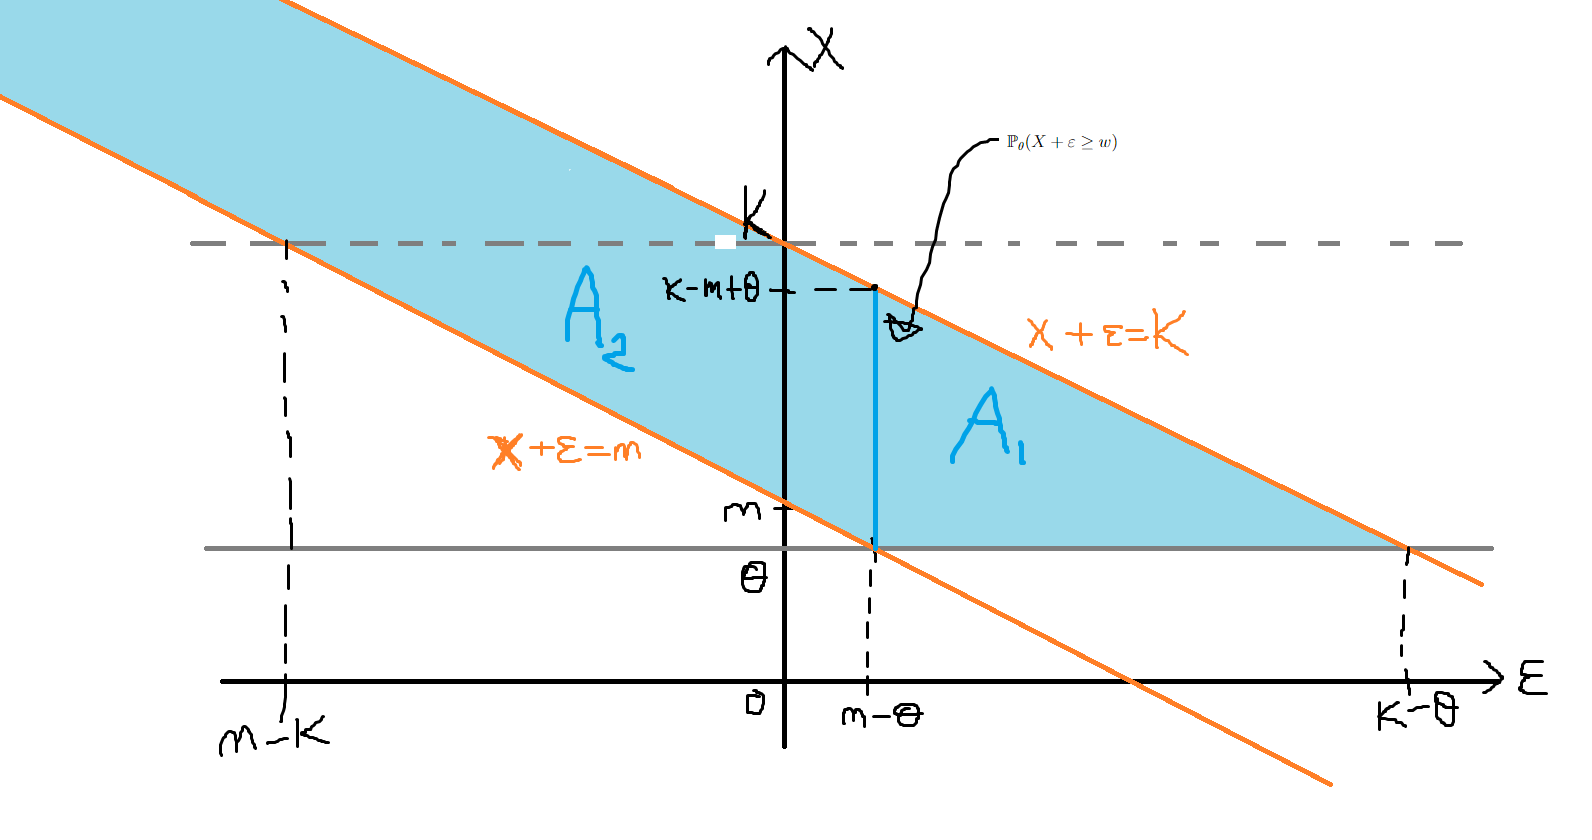
\includegraphics[width=\textwidth]{figures/minmi-integral-sketch.png}
    \caption{Sketch of the region to integrate over}
    \label{fig: minmi_integral}
\end{figure}

Let our statistic $S(\bm{W})$ be the minimum statistic $\min(W_1, \dots, W_n)$, $m = S(\bm{w})$ be the observed minimum, and $\theta_q$ be the $q\textsuperscript{th}$ quantile such that $\PP_{\theta_q} (S(\bm{W}) \geq m) = q$: \begin{align*}
    q &= \PP_{\theta_q} (S(\bm{W}) \geq m) \\
        &= \prod_{i=1}^n \PP_{\theta_q} (X_{i} + \varepsilon_i \geq m) \\
        &= \left[ 1 - \frac{F_\varepsilon(m-\theta_q)}{F_\varepsilon(K - \theta_q)} \psi(\theta_q; m)  \right]^n \\
    q^{\frac{1}{n}} &= 1 - \frac{F_\varepsilon(m-\theta_q)}{F_\varepsilon(K - \theta_q)} \psi(\theta_q; m) \numberthis \label{eqn: minmi-ee}
\end{align*}

The MINMI estimator $\hat\theta_q$ can be found using inversion by solving the above equation for $\theta = \hat\theta_q$. However, since $\psi$ does not simplify in general, we can approximate it with a Monte Carlo integral using $B$ samples, resulting in the below MINMI estimating equation: \begin{align*}
    q^{\frac{1}{n}} &= 1 - \frac{F_\varepsilon(m - \theta_q)}{F_\varepsilon(K - \theta_q)} \hat\psi_B(\theta_q; m); &\hat\psi_B(\theta_q; m) =  \frac{1}{B} \sum_{b=1}^B \frac{m-e_b-\hat\theta_q}{K-e_b-\theta_q} \numberthis \label{eqn: minmi-ee-mc}
\end{align*}

where $e_b$ are drawn from $f_\varepsilon(e_b)$ truncated at $m-\hat\theta_q$

As mentioned before, a requirement for inversion is for $\PP_{\theta} (M \geq m)$ to be stochastically increasing in $\theta$.

\subsection{Asymptotic Properties}

We now discuss the asymptotic properties of the MINMI estimator. The delta method gives the approximate result \begin{equation}
    \Var(\hat\theta_q) \approx \sigma^2_{\psi(\theta_q)} \left[ \frac{F(K-\theta_q)}{f(K-\theta) \hat\psi(\theta_q) + F(K-\theta) \hat\psi^\prime(\theta_q)} \right]^2
\end{equation}

The full proof of this result is provided in Appendix \ref{apx: minmi-asymptotics}. We were also able to verify these results empirically by simulation, generating estimates for upper and lower endpoints of a central $100(1-\alpha/2)\%$ confidence interval across different values of $B$.

\begin{figure}
    \centering
    \include{}
    \caption{Caption}
    \label{fig:my_label}
\end{figure}

\subsection{No Measurement Error}

If we assume measurement error is negligible, we may completely eliminate $\varepsilon$ from the above. Thus, the quantile estimate becomes trivial to find as $W = X$, which is uniformly distributed:
\begin{align*}
    \PP_\theta (M \geq m)
        &= \prod_{i=1}^n \PP_\theta (X_i \geq m) \\
        &= \left[ \PP_\theta (X_i \geq m) \right]^n, \quad \text{since our $X$'s are assumed i.i.d}\\
        &= \left( \frac{K - m}{K - \theta} \right)^n \\
    \implies q = \PP_{\hat{\theta}_q}(M \geq m) &= \left( \frac{K - m}{K - \hat{\theta}_q} \right)^n \\
    \therefore \hat{\theta}_q &= K - q^{-1/n} (K-m) \numberthis
\end{align*}
